% ------------------------------------------------------------------------------------------------
% koniec zadania 1 -------------------------------------------------------------------------------
% ------------------------------------------------------------------------------------------------

% MORE FUN UI STUFF
\begin{frame}[fragile]\frametitle{Pyszne tosty z masełkiem (android.widget.Toast)}

\begin{figure}[h]
 \centering
 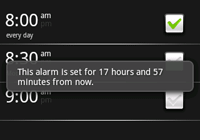
\includegraphics[height=0.40\textheight,keepaspectratio=true]{images/toast}
\end{figure}

 Przykład użycia: 
 \begin{lstlisting}
Toast.makeText(getApplicationContext(),
               "Halo Szczecin!", 
               Toast.LENGTH_LONG)
     .show();
 \end{lstlisting}

\end{frame}

\begin{frame}[fragile]
\frametitle{Co więcej potrafi Toast?}
\begin{lstlisting}
 Toast t = Toast.makeText(this, txt, LENGTH_SHORT);
\end{lstlisting}

\pause

Można mu zmienić pozycję:
\begin{lstlisting}
t.setGravity(Gravity.TOP|Gravity.LEFT, 0, 0);
\end{lstlisting}

\pause

lub podmienić widok:
\begin{lstlisting}
View customView = findViewById(R.id.custom_view);
/**/
t.setView(customView)
 \end{lstlisting}

\end{frame}

